\subsection{Workflow}
\par Nell'utilizzo di ChatSQL, il flusso più comune da seguire per ottenere una query \glossario{SQL} è:
\begin{enumerate}
  \item Accedere alla pagina Chat selezionandola dal menu di navigazione principale;
  \item Selezionare il \glossario{dizionario dati} desiderato;
  \item Selezionare il \glossario{DBMS} desiderato;
  \item Selezionare la lingua desiderata;
  \item Inserire una richiesta in linguaggio naturale e attendere la generazione del \glossario{prompt};
  \item Copiare il prompt generato cliccando sull'apposito pulsante in alto a destra all'interno del messaggio fornito dal ChatBOT;
  \item Incollare il prompt in un modello \glossario{LLM} a scelta (come ChatGPT) e attendere la generazione della query SQL.
\end{enumerate}

\vspace{\baselineskip}
\par Di seguito è riportata una figura che illustra nel dettaglio il flusso da seguire per ottenere una query SQL da utilizzare per interrogare \glossario{database} reali.

\begin{figure}[H]
  \fbox{
  \begin{tabular}{cc}
    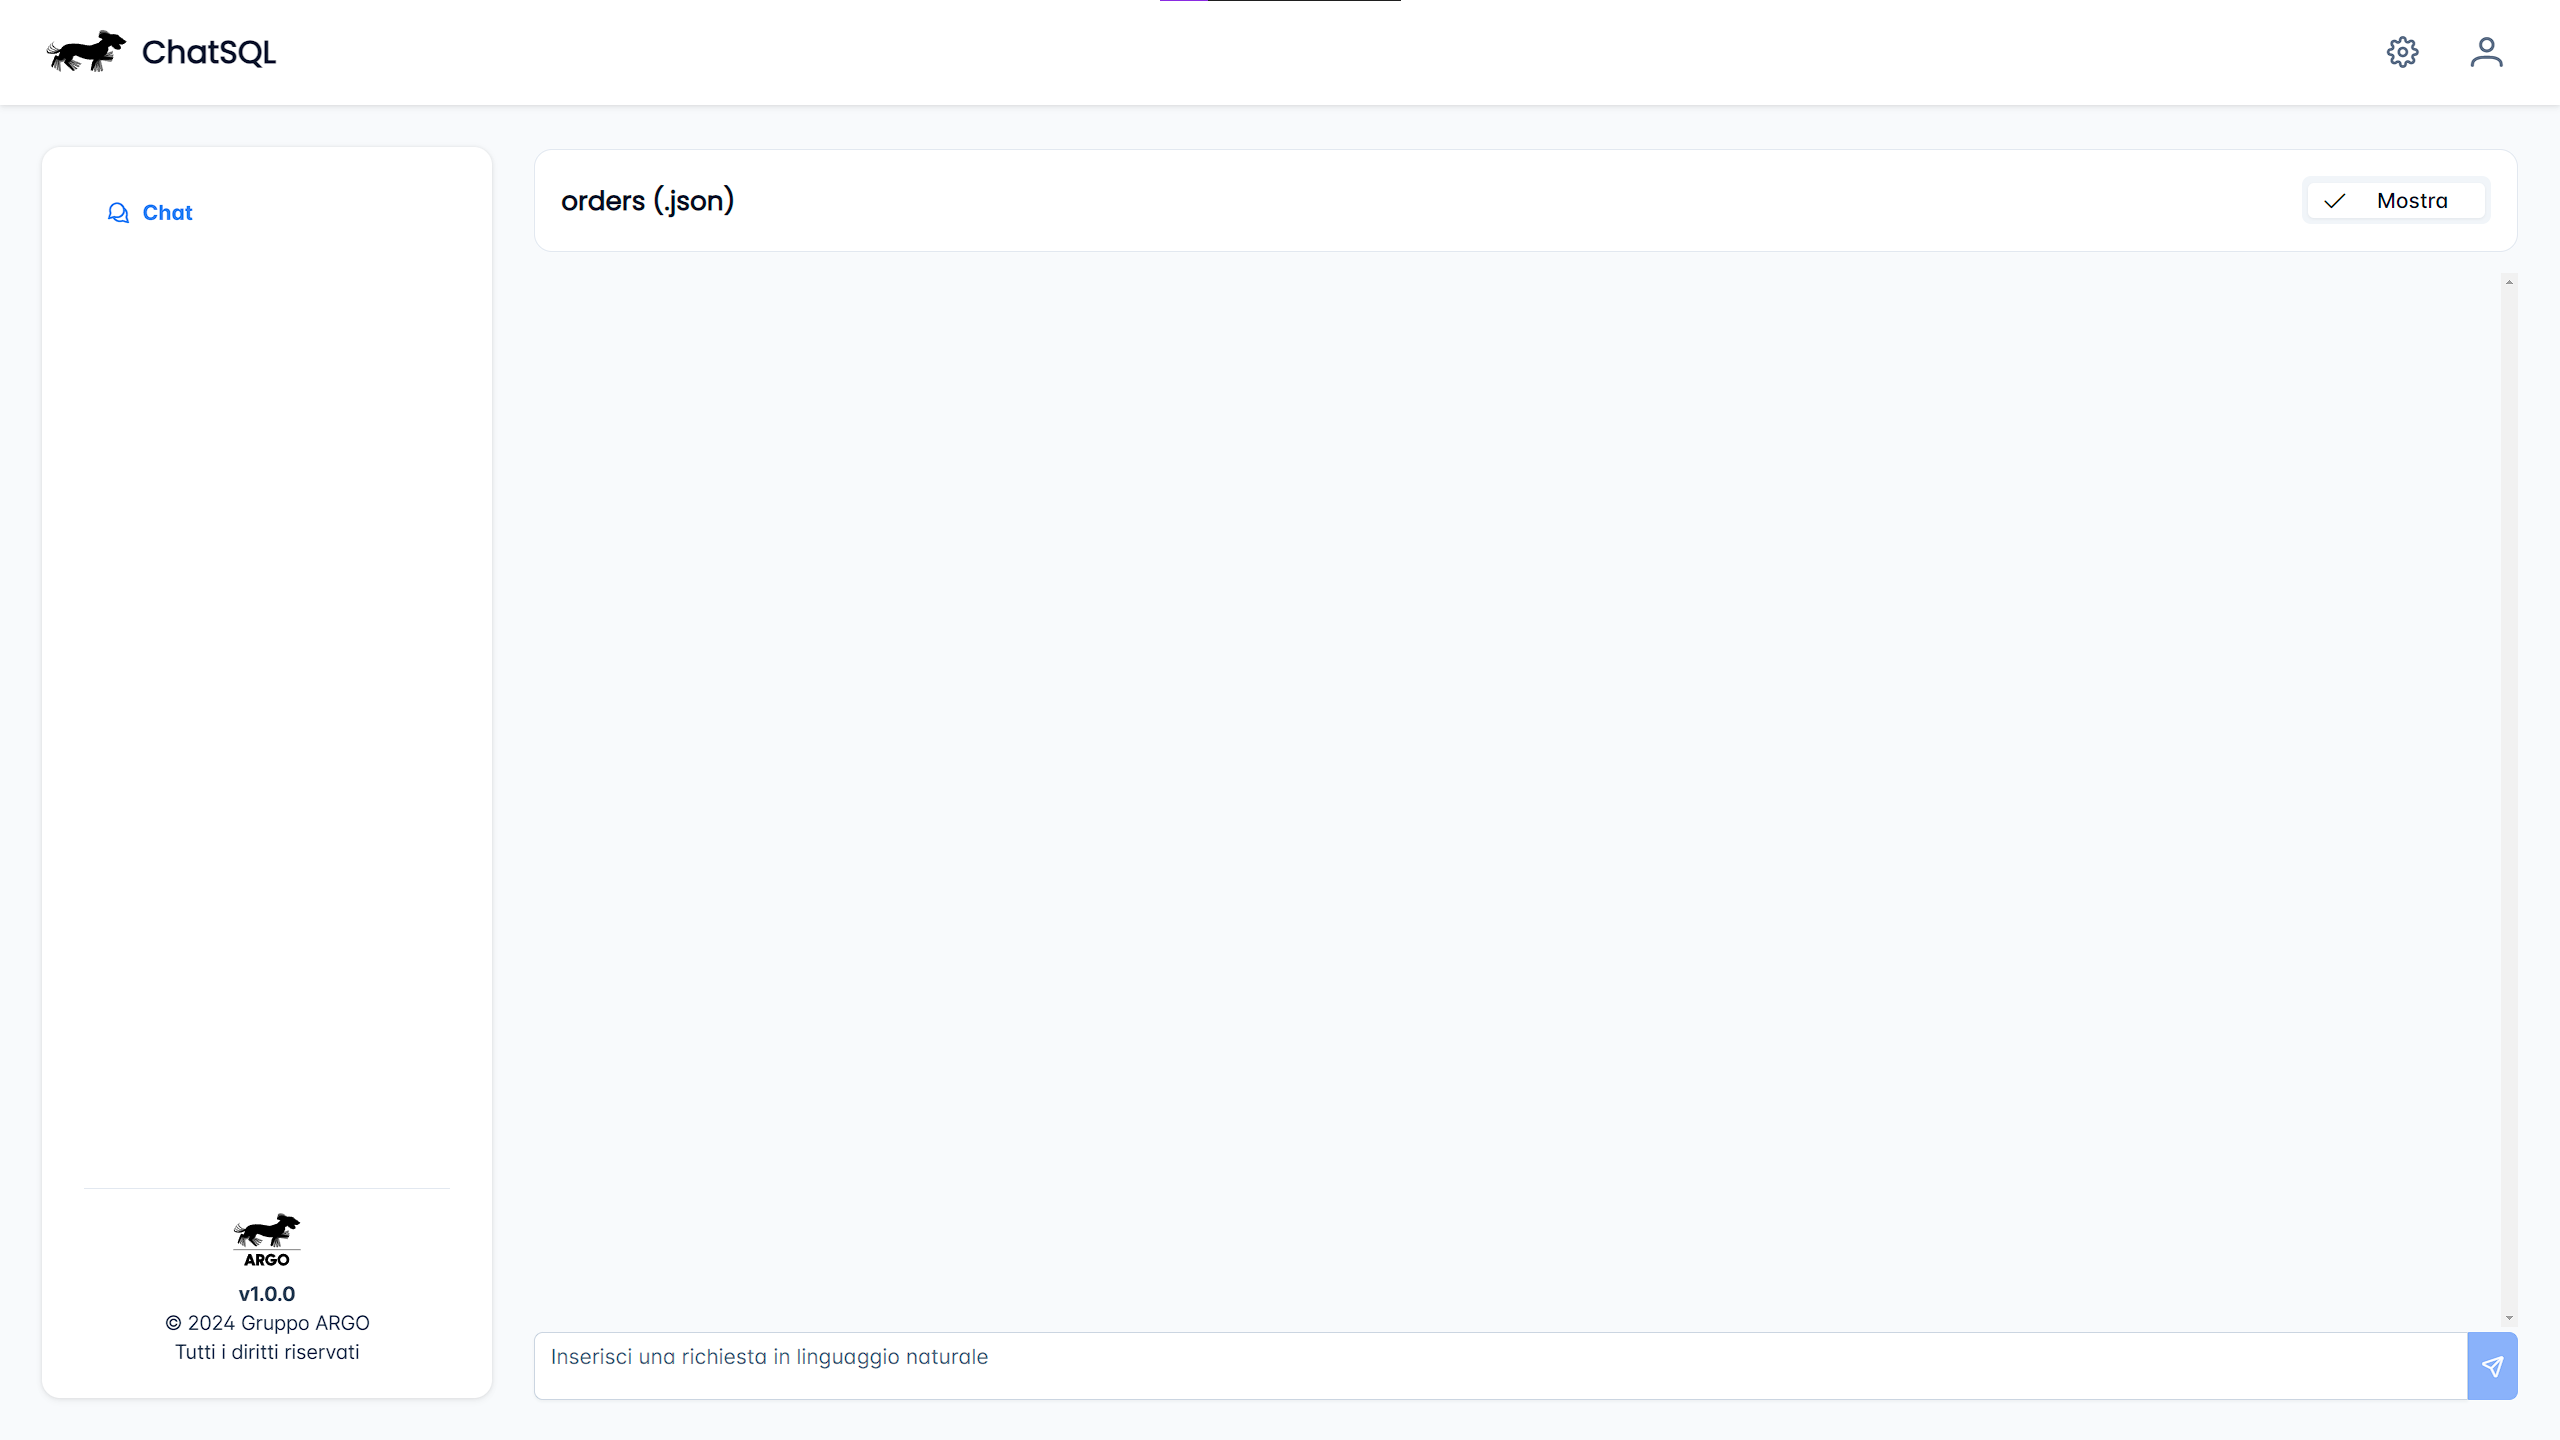
\includegraphics[width=65mm]{assets/workflow_1.png} &   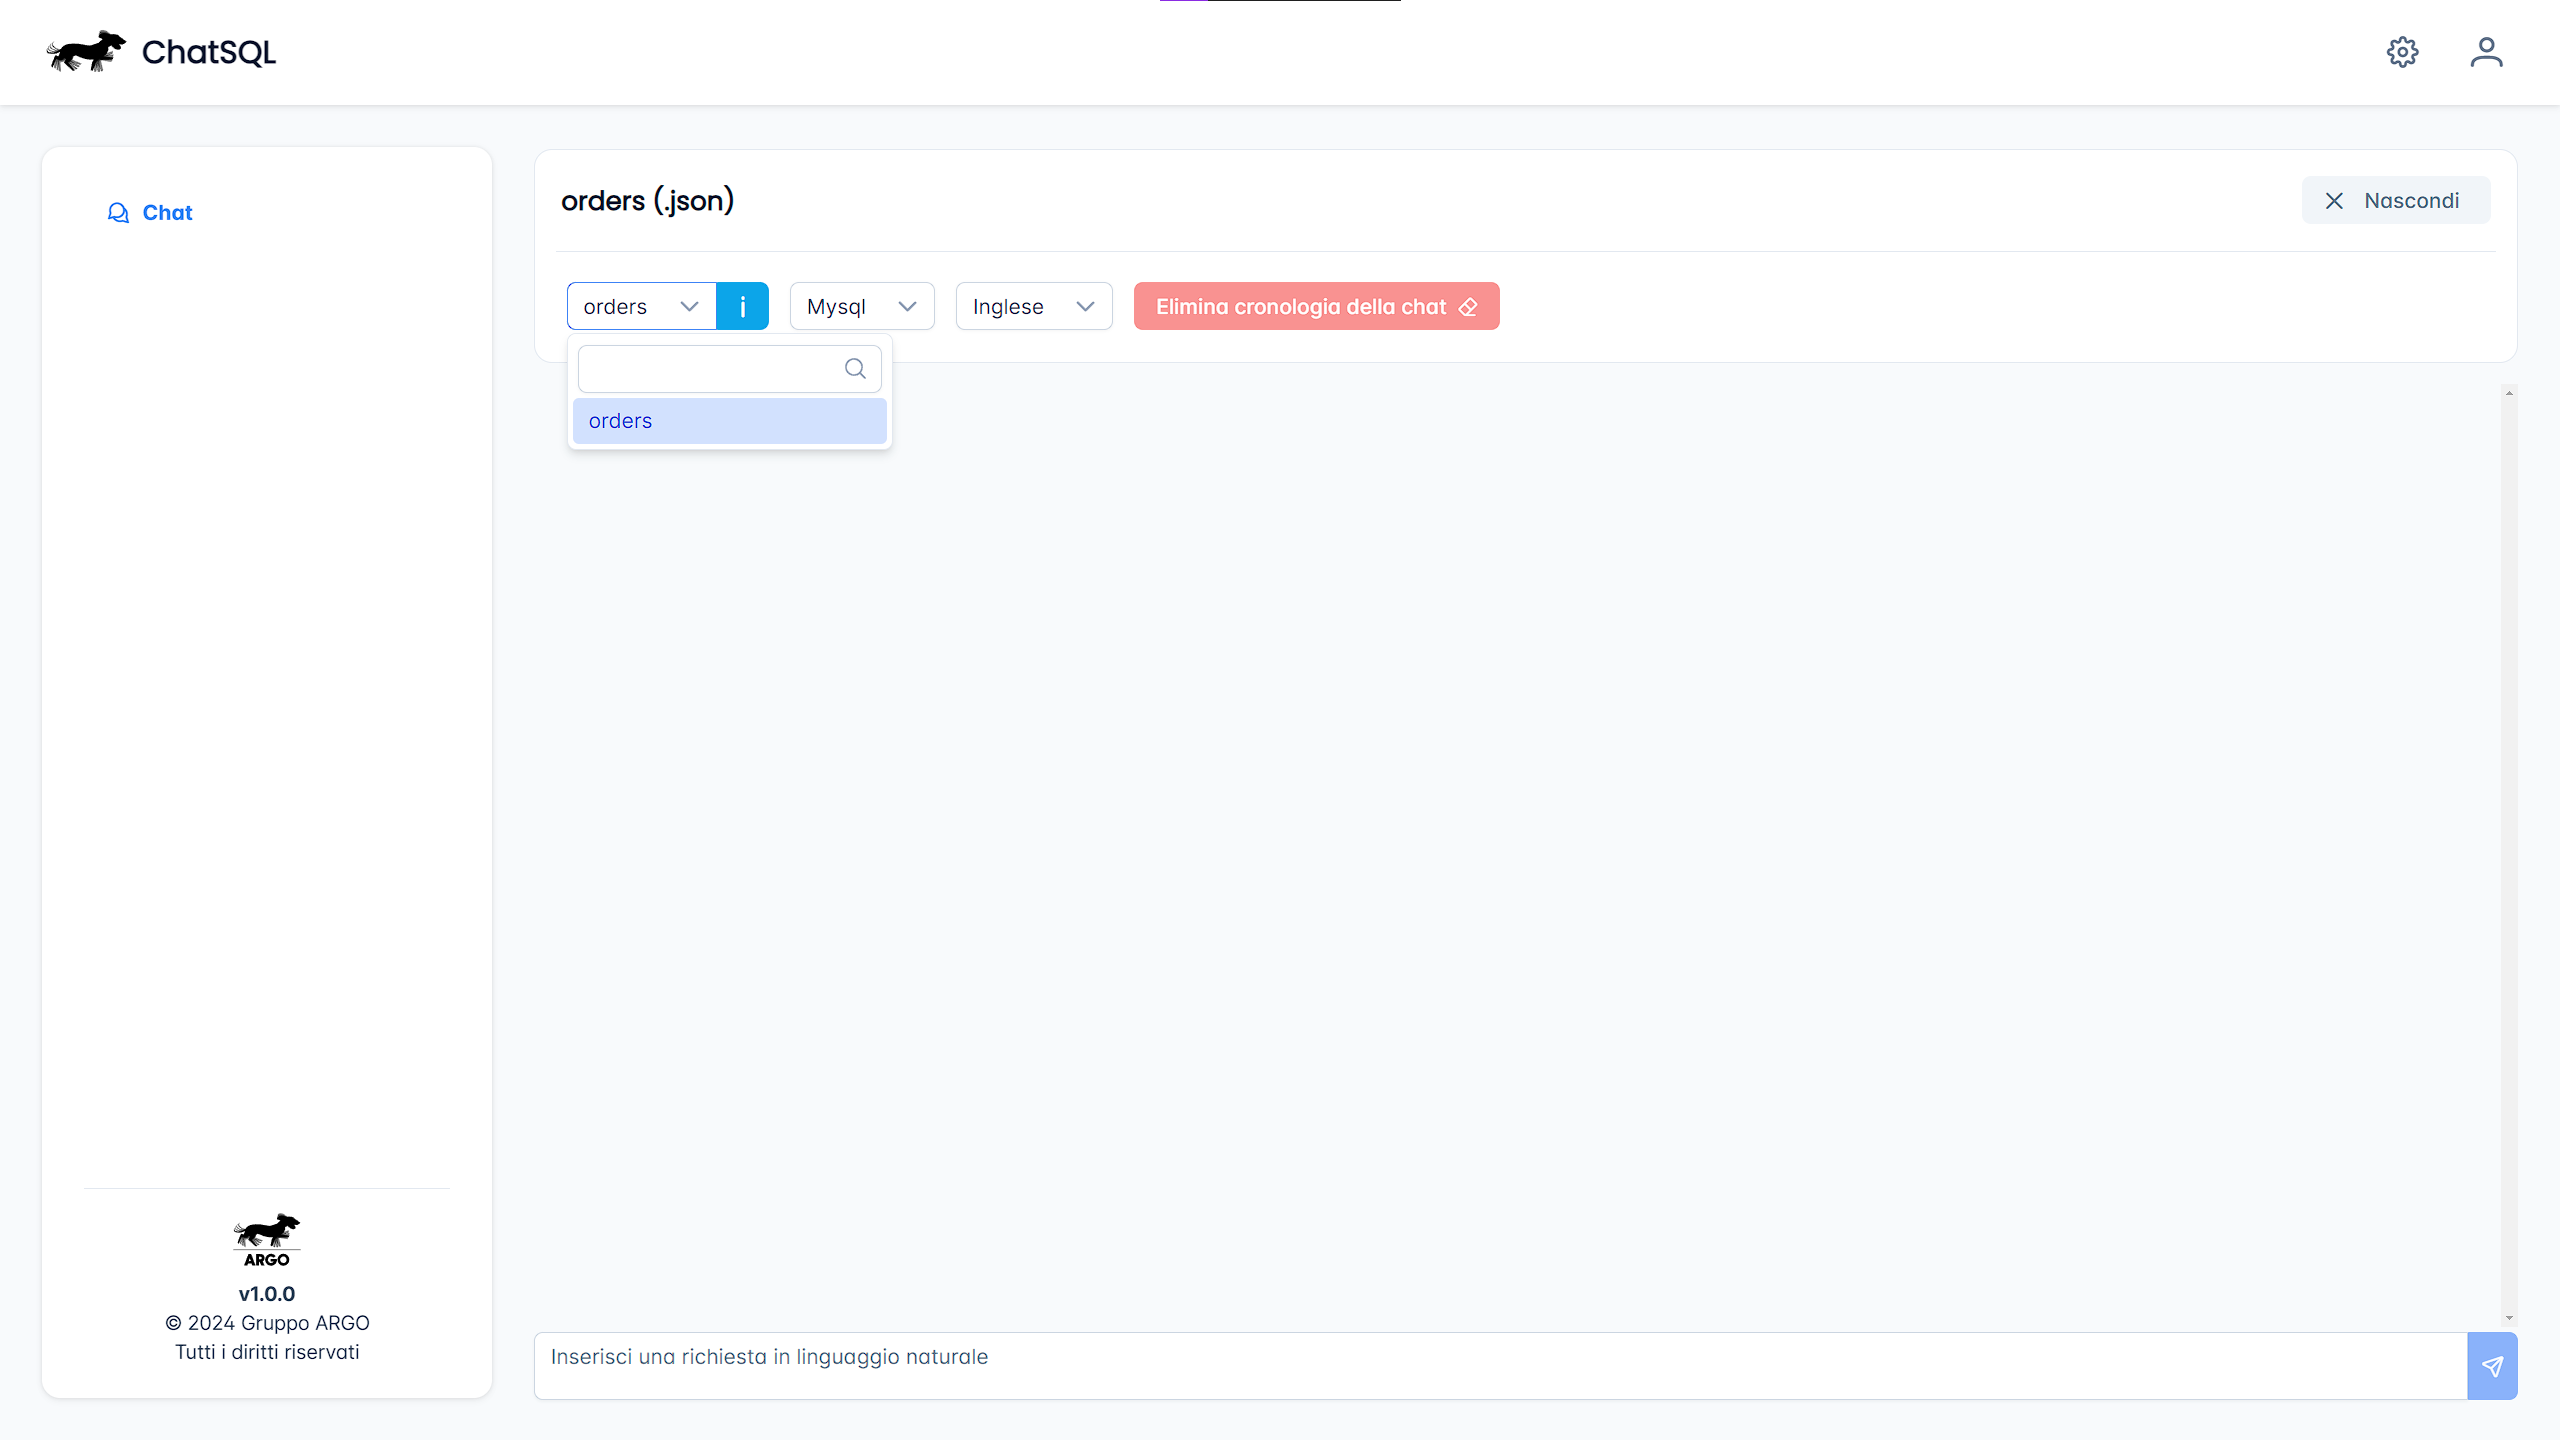
\includegraphics[width=65mm]{assets/workflow_2.png} \\
    1 & 2 \\[6pt]
     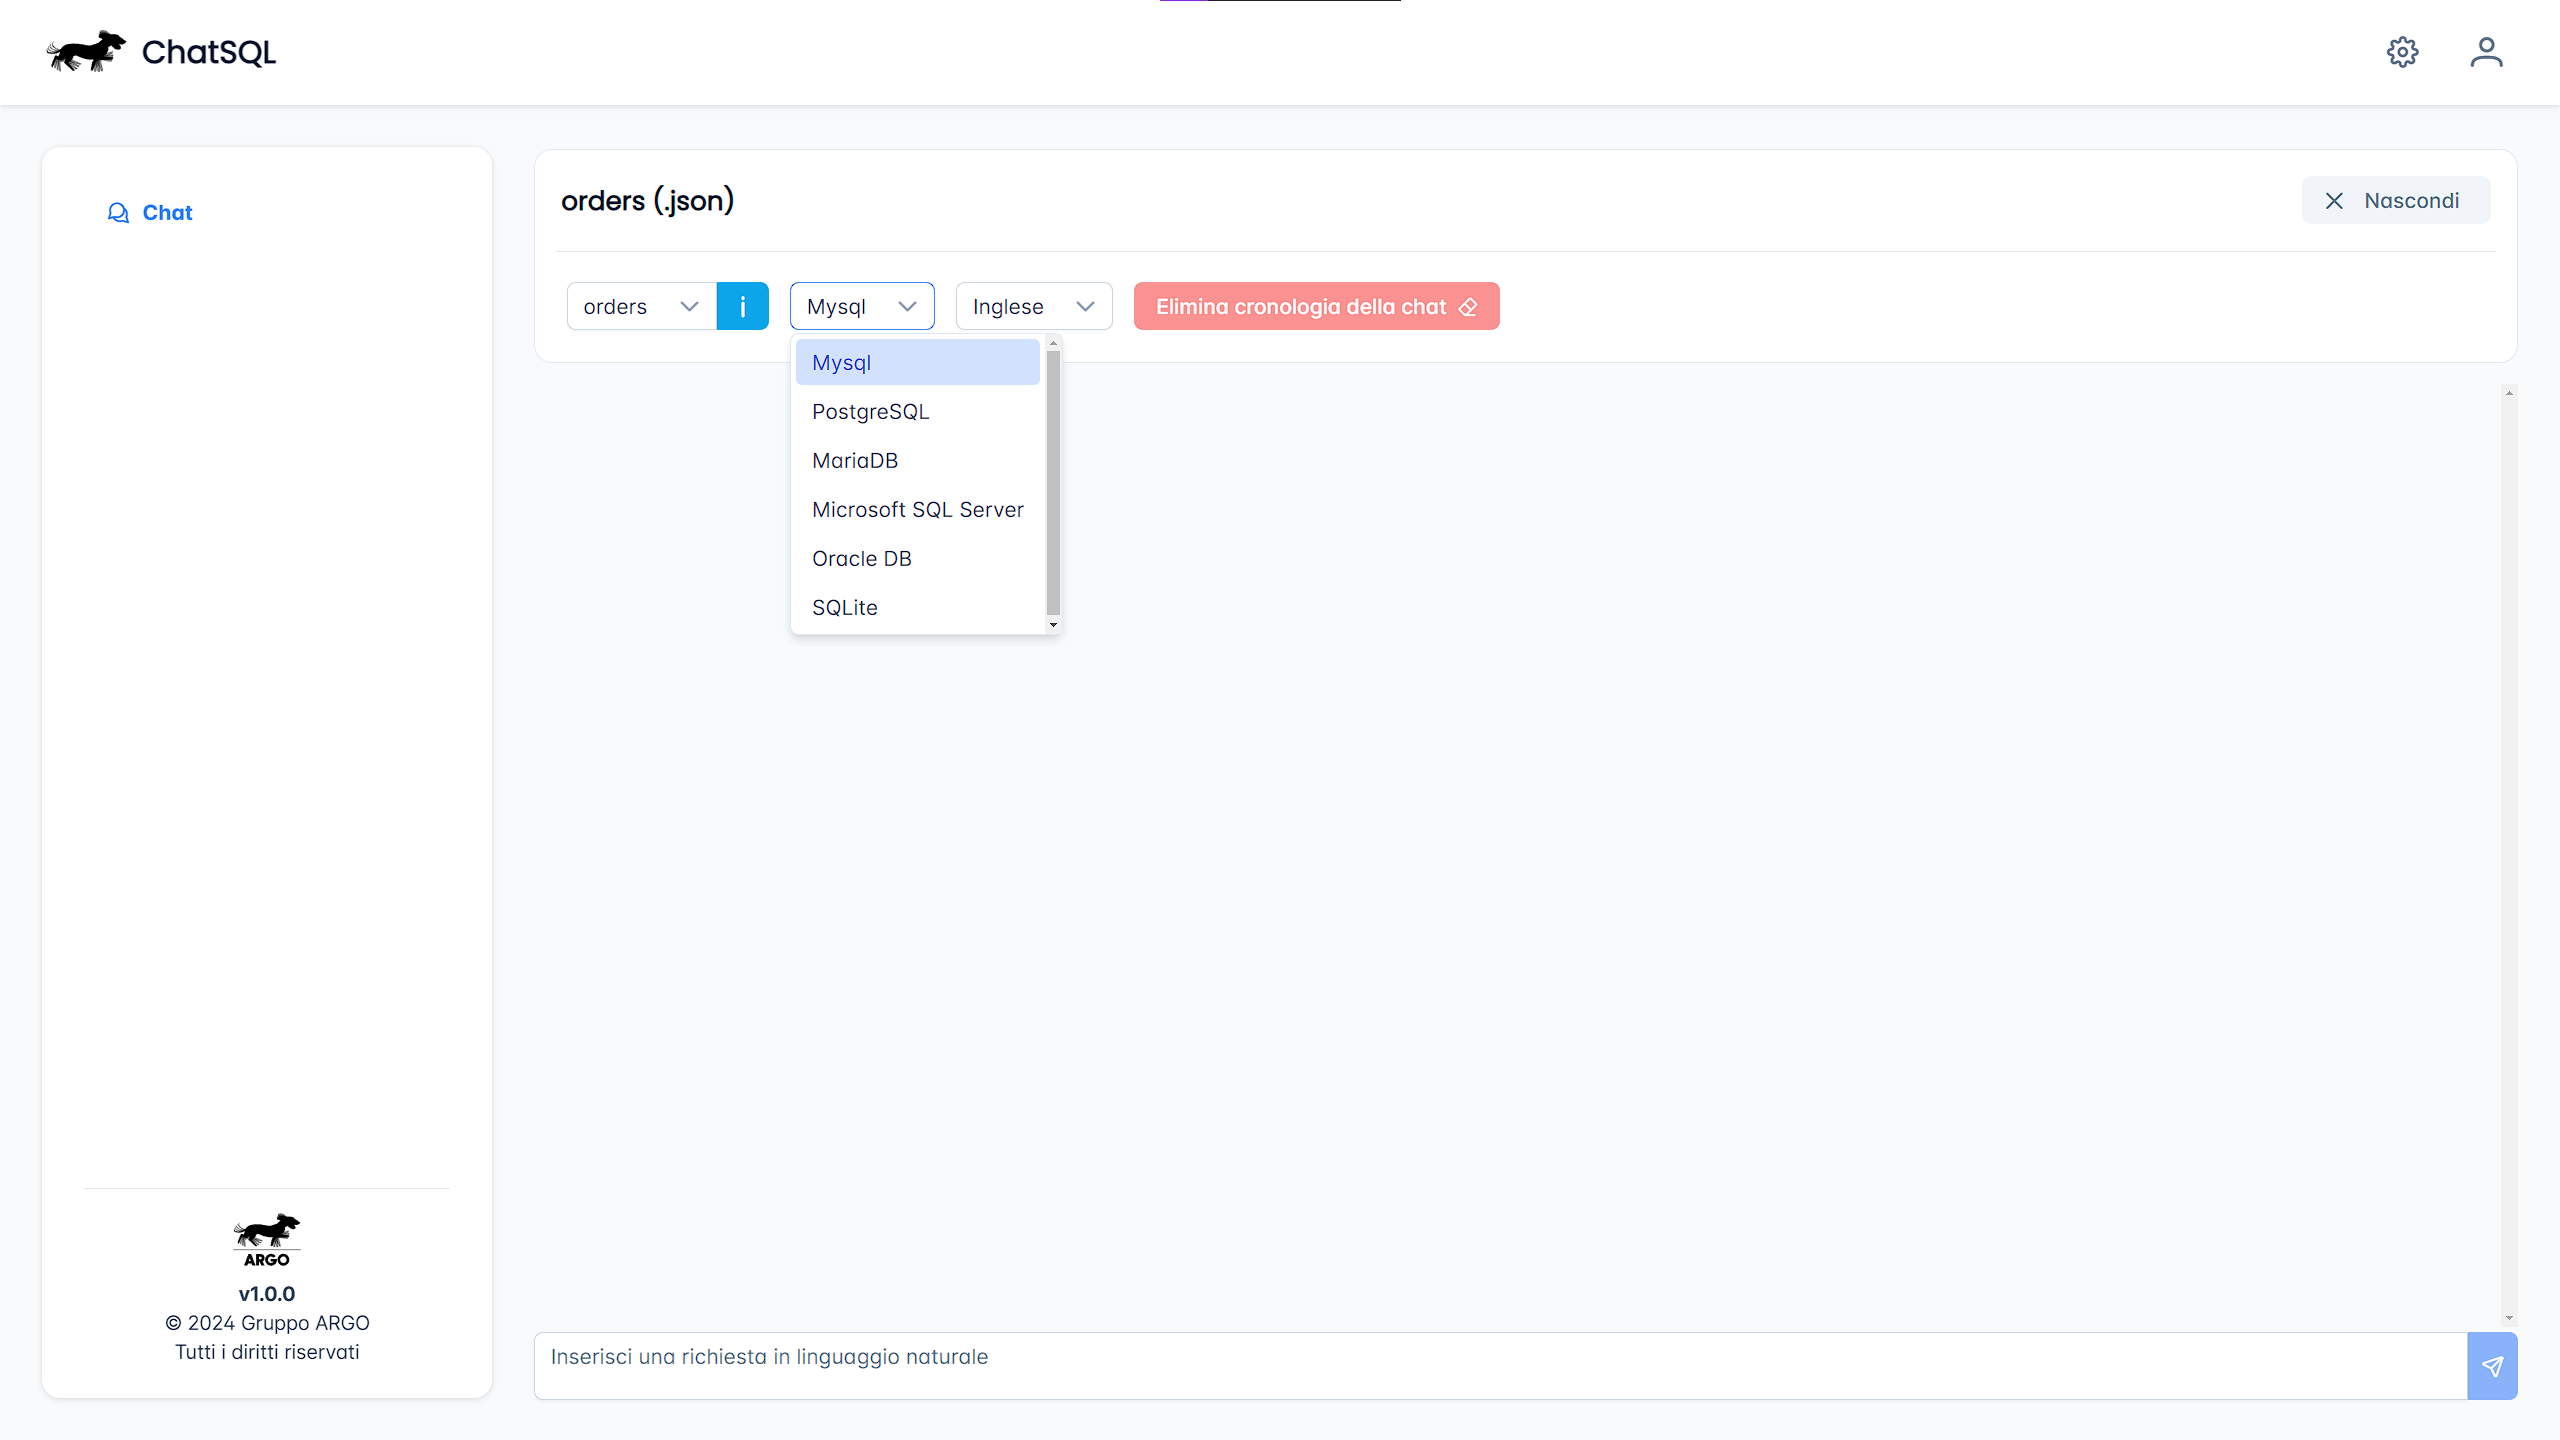
\includegraphics[width=65mm]{assets/workflow_3.png} &   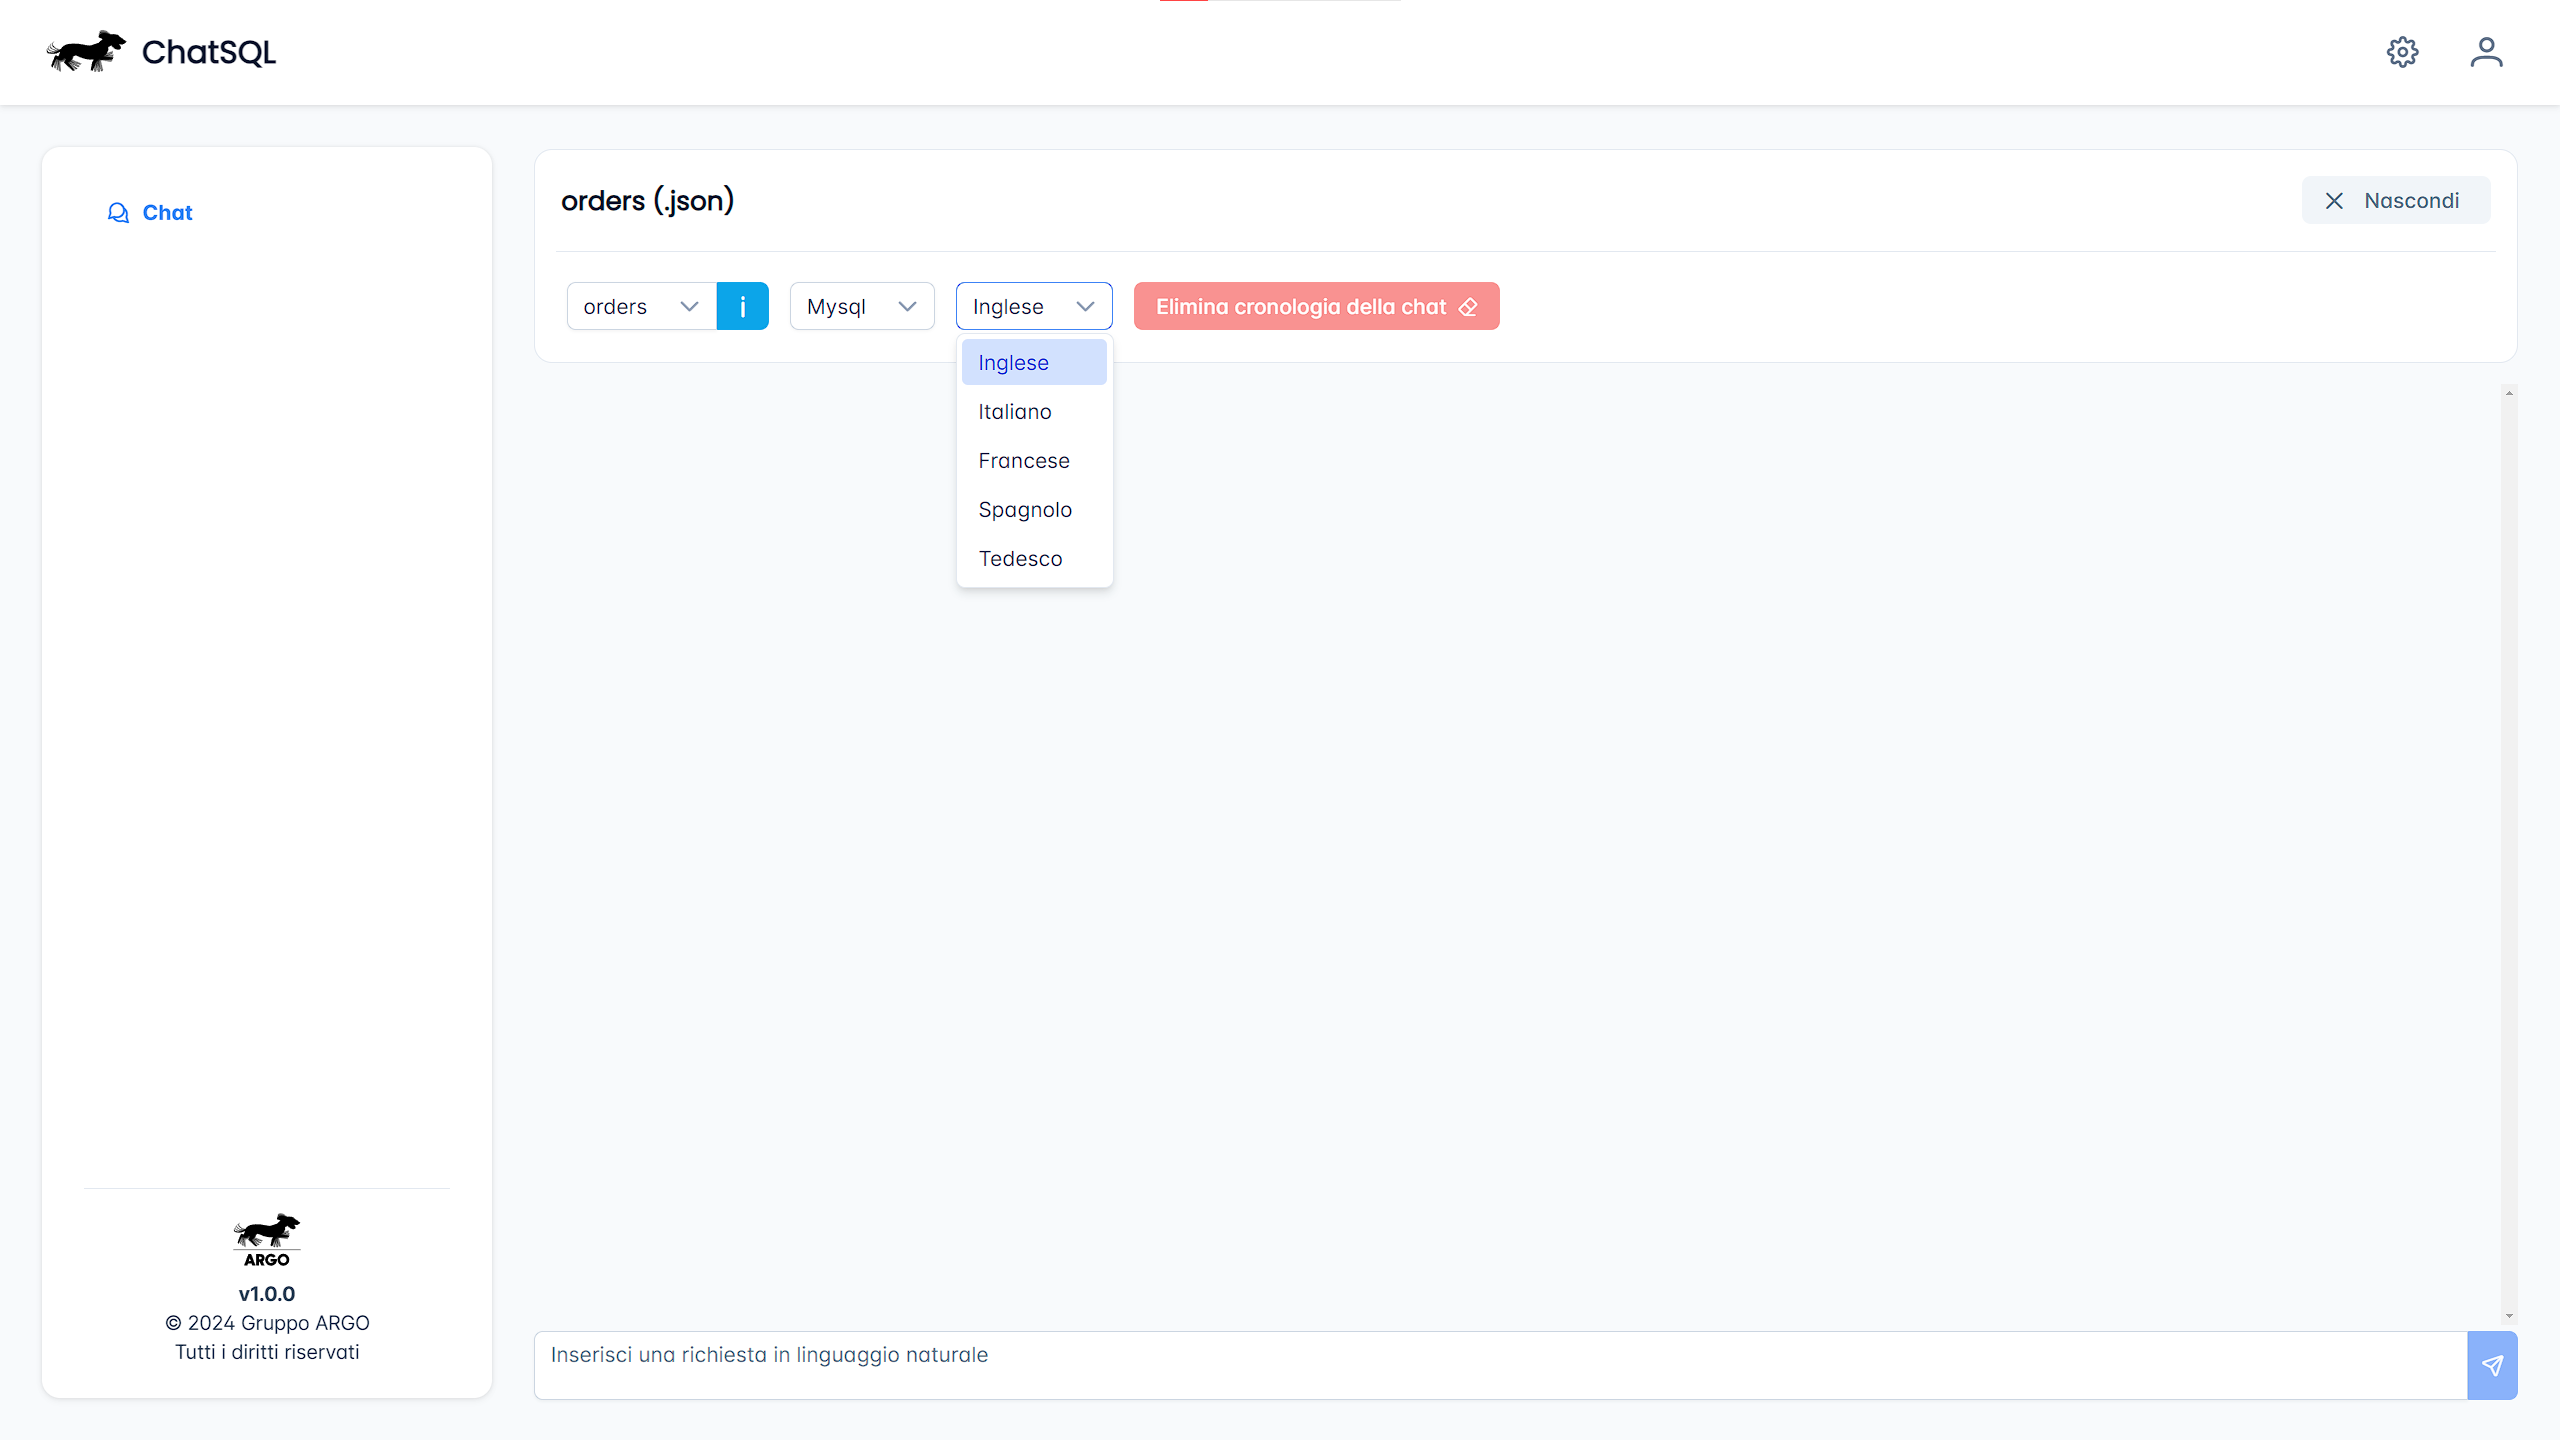
\includegraphics[width=65mm]{assets/workflow_4.png} \\
    3 & 4 \\[6pt]
   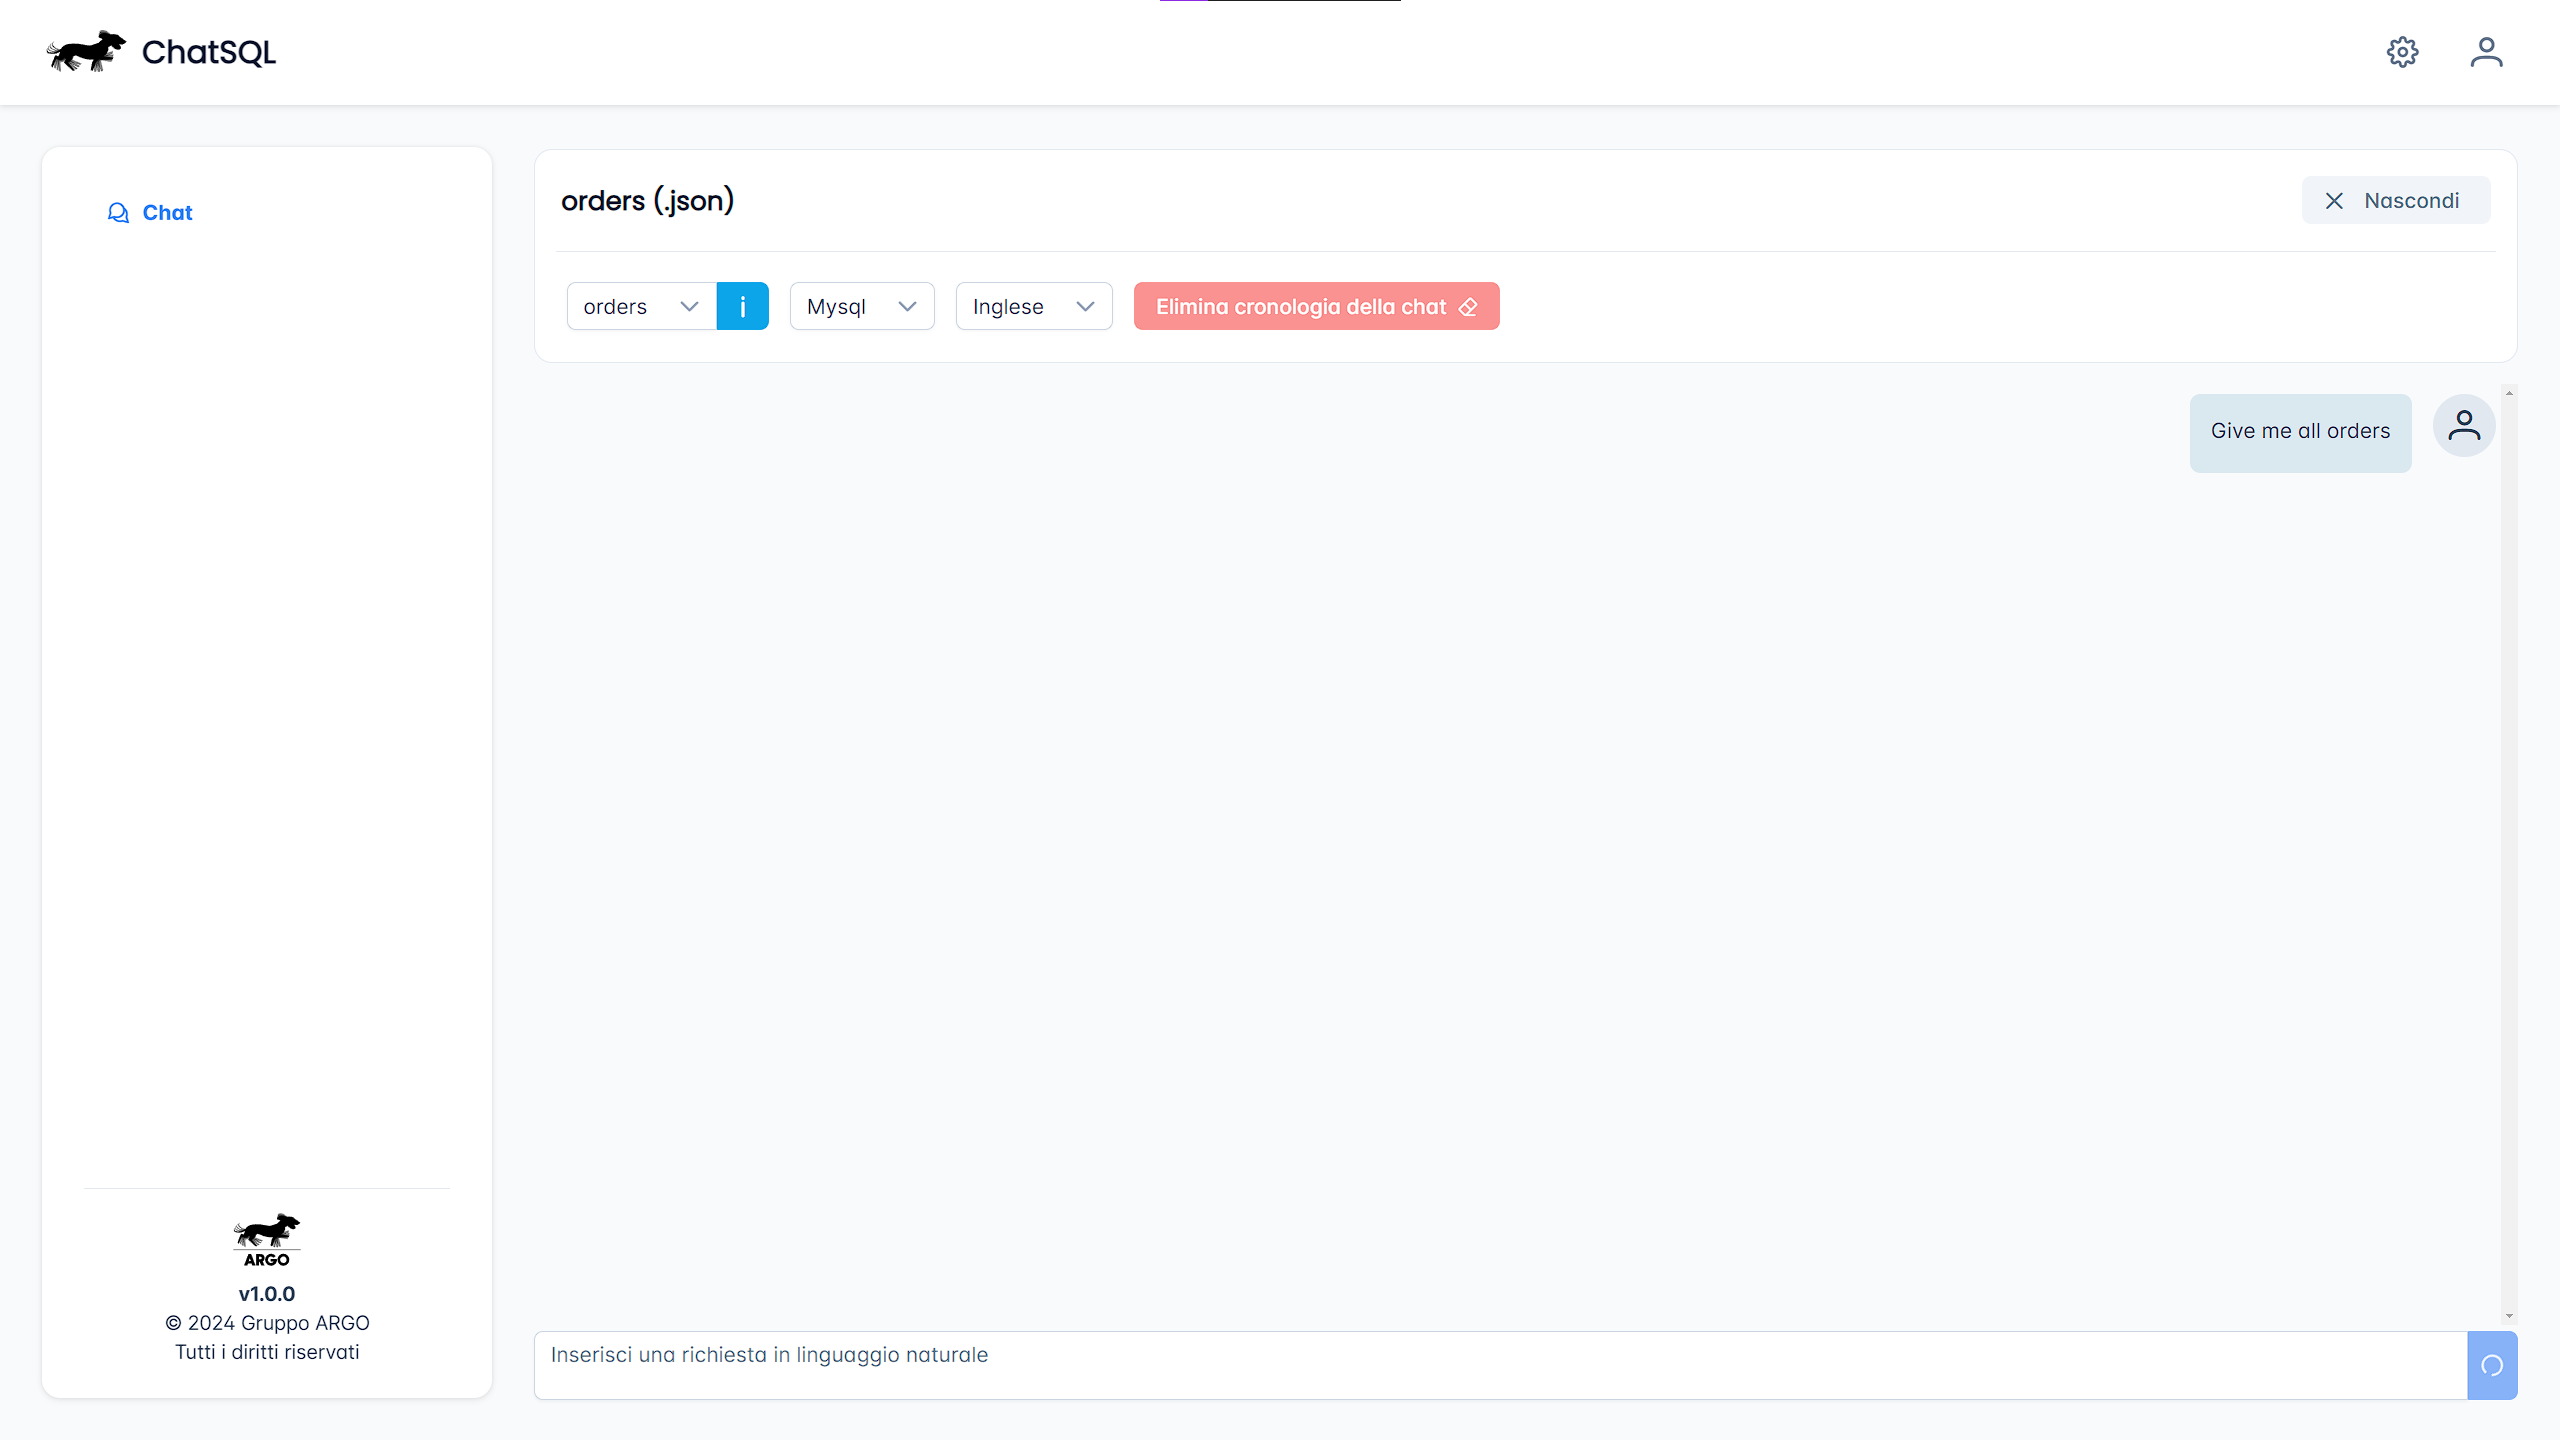
\includegraphics[width=65mm]{assets/workflow_5.png} &   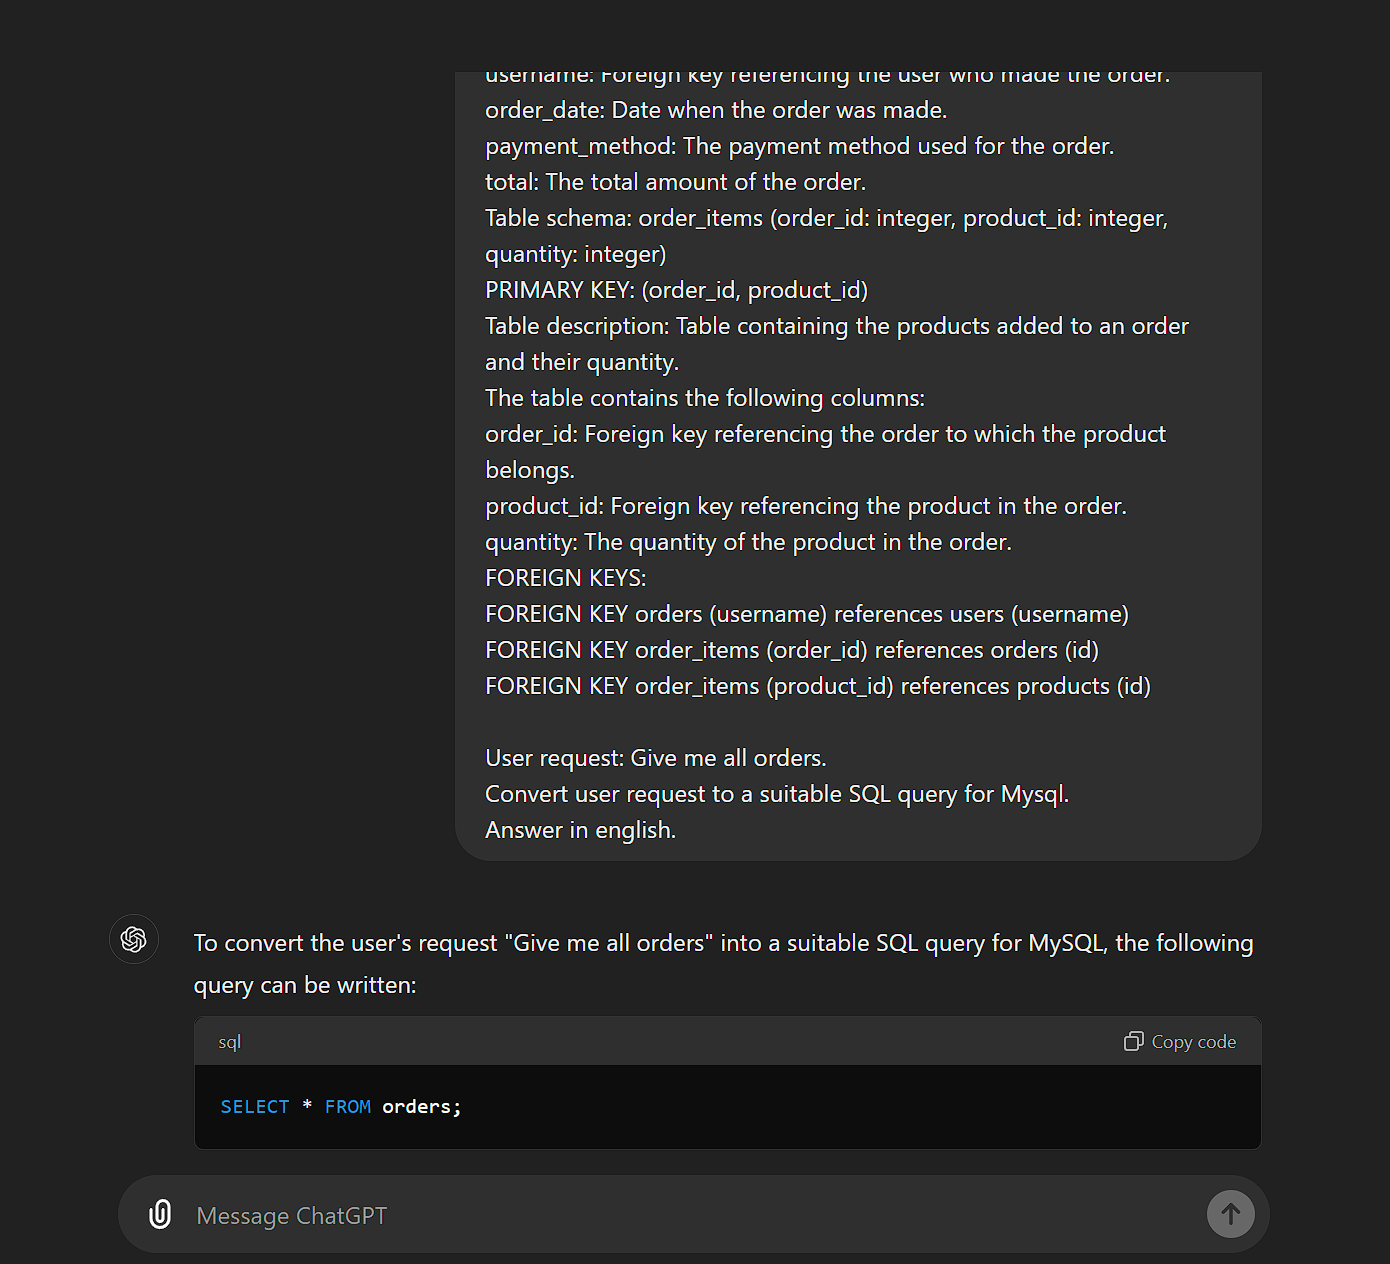
\includegraphics[width=65mm]{assets/workflow_6.png} \\
    5 & 6 \\[6pt]
    \multicolumn{2}{c}{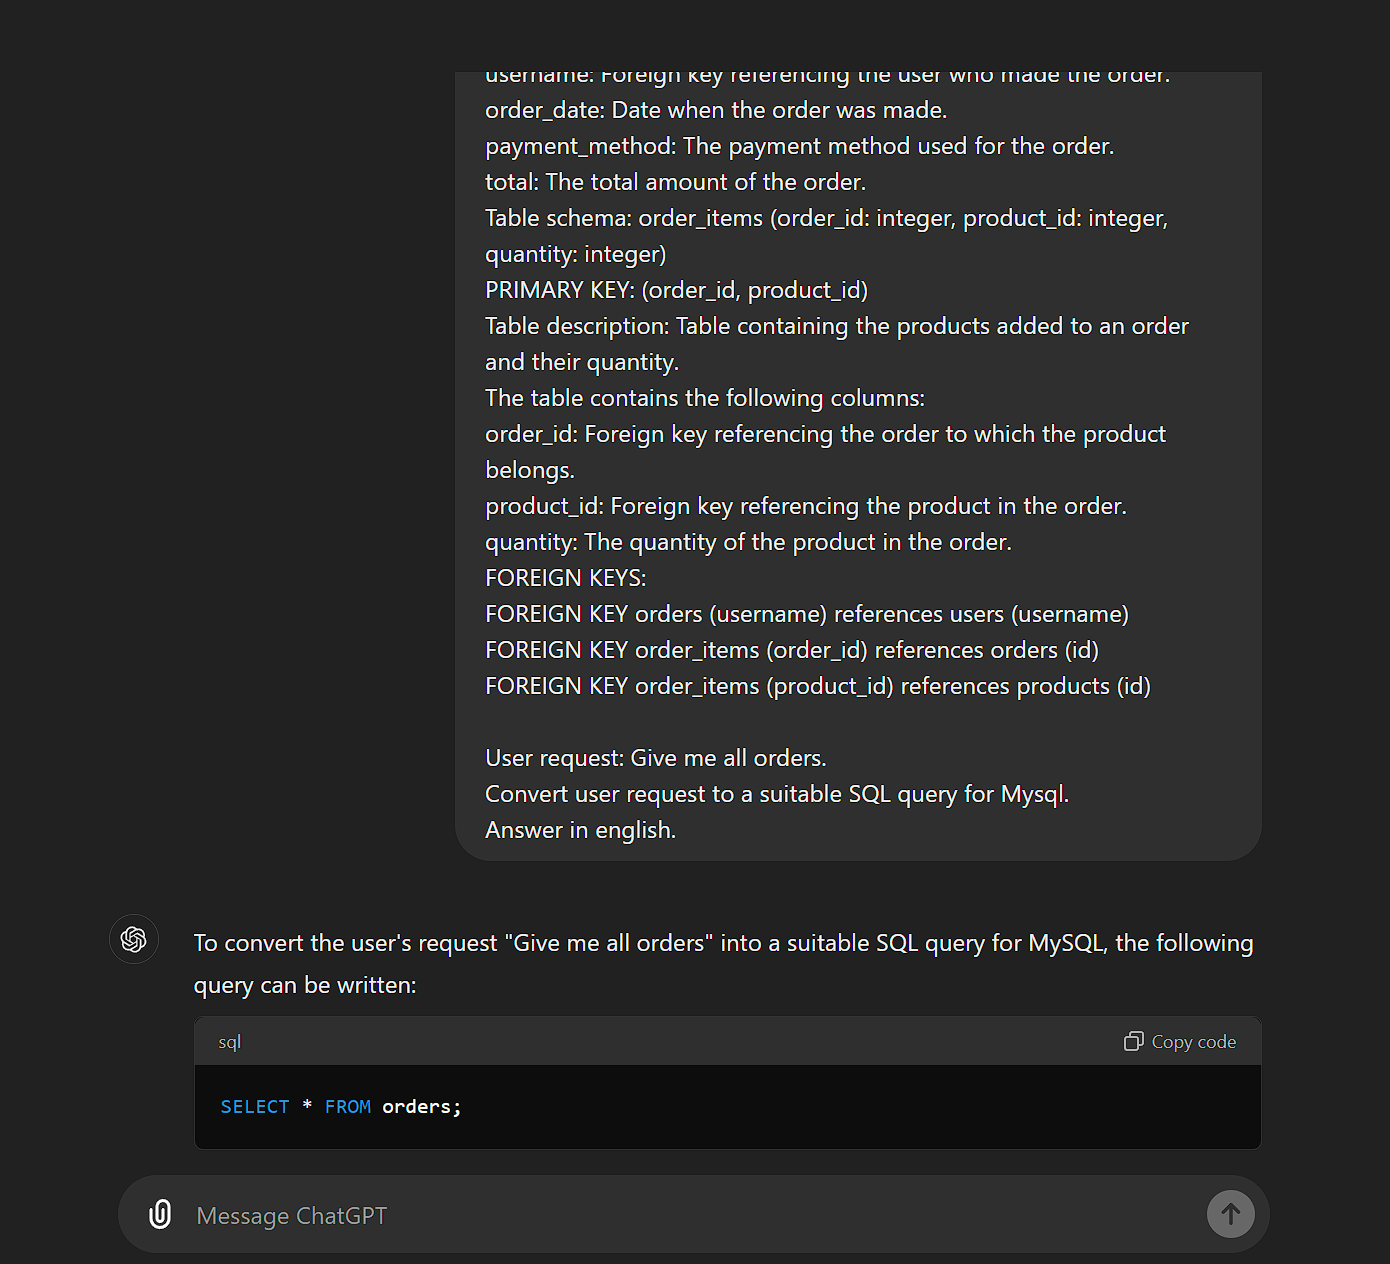
\includegraphics[width=65mm]{assets/workflow_7.png}}\\
    \multicolumn{2}{c}{7}
  \end{tabular}}
  \caption{Workflow per ottenere una query SQL}
\end{figure}
\par L'output atteso dal modello LLM è una query SQL che soddisfa la richiesta inserita, che potrà essere eseguita su un DBMS per ottenere i risultati desiderati.